% This example is meant to be compiled with lualatex or xelatex
% The theme itself also supports pdflatex
\PassOptionsToPackage{unicode}{hyperref}
\documentclass[aspectratio=1610, 12pt]{beamer}

% Warning, if another latex run is needed
% \usepackage[aux]{rerunfilecheck}

% just list chapters and sections in the toc, not subsections or smaller
\setcounter{tocdepth}{1}

%------------------------------------------------------------------------------
%------------------------------ Fonts, Unicode, Language ----------------------
%------------------------------------------------------------------------------
\usepackage{fontspec}
\defaultfontfeatures{Ligatures=TeX}  % -- becomes en-dash etc.

% german language
\usepackage{polyglossia}
\setdefaultlanguage{german}

% for english abstract and english titles in the toc
\setotherlanguages{english}

% intelligent quotation marks, language and nesting sensitive
\usepackage[autostyle]{csquotes}

% microtypographical features, makes the text look nicer on the small scale
\usepackage{microtype}

%------------------------------------------------------------------------------
%------------------------ Math Packages and settings --------------------------
%------------------------------------------------------------------------------

\usepackage{amsmath}
\usepackage{amssymb}
\usepackage{mathtools}
\usepackage{bbold}

% Enable Unicode-Math and follow the ISO-Standards for typesetting math
\usepackage[
  math-style=ISO,
  bold-style=ISO,
  sans-style=italic,
  nabla=upright,
  partial=upright,
]{unicode-math}
\setmathfont{Latin Modern Math}

% nice, small fracs for the text with \sfrac{}{}
\usepackage{xfrac}


%------------------------------------------------------------------------------
%---------------------------- Numbers and Units -------------------------------
%------------------------------------------------------------------------------

\usepackage[
  locale=DE,
  separate-uncertainty=true,
  per-mode=symbol-or-fraction,
]{siunitx}
\sisetup{math-micro=\text{µ},text-micro=µ}
% \sisetup{tophrase={{ to }}}
%------------------------------------------------------------------------------
%-------------------------------- tables  -------------------------------------
%------------------------------------------------------------------------------

\usepackage{booktabs}       % \toprule, \midrule, \bottomrule, etc

%------------------------------------------------------------------------------
%-------------------------------- graphics -------------------------------------
%------------------------------------------------------------------------------

\usepackage{graphicx}
%\usepackage{rotating}
\usepackage{grffile}
\usepackage{tikz}
\usepackage{circuitikz}
\usepackage{tikz-feynman}
\usepackage{subcaption}

% allow figures to be placed in the running text by default:
\usepackage{scrhack}
\usepackage{float}
\floatplacement{figure}{htbp}
\floatplacement{table}{htbp}

% keep figures and tables in the section
\usepackage[section, below]{placeins}

% smileys
\usepackage{MnSymbol,wasysym}

%------------------------------------------------------------------------------
%---------------------- customize list environments ---------------------------
%------------------------------------------------------------------------------

\usepackage{enumitem}
\usepackage{listings}
\usepackage{hepunits}

\usepackage{pdfpages}
%------------------------------------------------------------------------------
%------------------------------ Bibliographie ---------------------------------
%------------------------------------------------------------------------------

\usepackage[
  backend=biber,   % use modern biber backend
  autolang=hyphen, % load hyphenation rules for if language of bibentry is not
                   % german, has to be loaded with \setotherlanguages
                   % in the references.bib use langid={en} for english sources
]{biblatex}
\addbibresource{references.bib}  % the bib file to use
\DefineBibliographyStrings{german}{andothers = {{et\,al\adddot}}}  % replace u.a. with et al.


% Load packages you need here
% \usepackage{polyglossia}
% \setmainlanguage{german}

\usepackage{csquotes}


% \usepackage{amsmath}
% \usepackage{amssymb}
% \usepackage{mathtools}

\usepackage{hyperref}
\usepackage{bookmark}

% load the theme after all packages

\usetheme[
  showtotalframes, % show total number of frames in the footline
]{tudo}

% Put settings here, like
\unimathsetup{
  math-style=ISO,
  bold-style=ISO,
  nabla=upright,
  partial=upright,
  mathrm=sym,
}

% \setbeamertemplate{itemize item}{\scriptsize$\blacktriangleright$}
% \setbeamertemplate{itemize subitem}{\scriptsize$\blacktriangleright$}

%Titel:
\title{Joint constraints for SciFi modules alignment}
\subtitle{tuning of uncertainties}
%Autor
\author[N.Breer]{Nils Breer}
%Lehrstuhl/Fakultät
\institute{TU Dortmund, AG Albrecht}
%\titlegraphic{\includegraphics[width=0.3\textwidth]{content/Bilder/interferenz.jpg}}
% \date{12.05.2023}

\begin{document}
\maketitle

\begin{frame}\frametitle{Concept for joint constraint}
  \begin{columns}
    \begin{column}[c]{0.65\textwidth}
      \begin{itemize}
        \setlength\itemsep{0em}
        \item $\bullet$\, Long SciFi modules: slight "banana shape"
        \item $\bullet$\, Half modules + joints reproduce the real shape
        \item $\bullet$\, Joints are implemented in the alignment by using a survey constraint (\href{https://gitlab.cern.ch/lhcb/Alignment/-/merge_requests/368}{MR!368})
        \item $\bullet$\, It constrains  parameters of two alignables A and B to each other with a $chi^2$: $\chi^2 = (p_A - p_B)^T\,V^{-1}\,(p_A - p_B)$
        \item $\bullet$\, $p_A, p_B$: set of parameters for the half modules
        \item $\bullet$\, Use common frame (local half module frame)
        \item $\bullet$\, Errors taken from diagonal covariance matrix \to how realistic? \to tuning needed
        \item $\bullet$\, No survey available for joints, tuning needed to contol their $\chi^2$
      \end{itemize}
    \end{column}
    \begin{column}[c]{0.35\textwidth}
      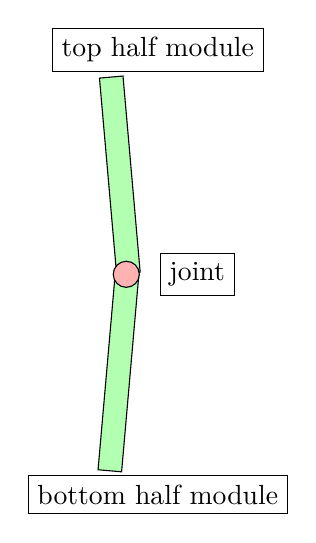
\begin{tikzpicture}
    \node[rectangle, 
    draw = black, 
    fill = green!30!white, 
    minimum width = 0.3cm, 
    minimum height = 2.5cm,
    rotate around = {-5:(0,0)}] at (0,0) {};
    \node[rectangle, 
    draw = black, 
    fill = green!30!white, 
    minimum width = 0.3cm, 
    minimum height = 2.5cm,
    rotate around = {5:(0,2.5)}] at (-0.2,2.5) {};
    \node[circle, 
    draw = black, 
    fill = red!30!white, 
    minimum width = 0.01cm] at (0.1,1.25) {};

    \node[draw, align=left] at (0.5, 4.1) {top half module};
    \node[draw, align=left] at (1, 1.25) {joint};
    \node[draw, align=left] at (0.5, -1.55) {bottom half module};
\end{tikzpicture}
    \end{column}
  \end{columns}
\end{frame}

\begin{frame}\frametitle{Tuning procedure}
  \begin{columns}
    \begin{column}[c]{0.48\textwidth}
      \begin{itemize}
        \item $\bullet$\, Instead of one $\chi^2$ for whole cov. matrix \to look at the $\chi^2$ for joint parameters (Tx,Ty,Tz,Rx,Ry,Rz)
        \item $\bullet$\, \href{https://gitlab.cern.ch/lhcb/Alignment/-/blob/master/Alignment/TAlignment/src/AlignChisqConstraintTool.cpp}{AlignChisqConstraintTool.cpp} was modified to  calculate the six $chi^2$ values to the software (MR coming soon)
        \item $\bullet$\, Tune uncertainties by running an alignment for each change to the respective parameter uncertainty until roughly $\chi^2 / \text{dof} = 1$
        % \item $\bullet$\, using $\chi^2$ to learn about accuracy of the joint constraint errors
      \end{itemize}
    \end{column}
    \begin{column}[c]{0.48\textwidth}
      \begin{itemize}
        \item $\bullet$\, Procedure evaluated with 2023 data (run 269045, warm SciFi) and master from conditions database
        \item $\bullet$\, Using the Alignment master branch
      \end{itemize}
      \begin{figure}
        \includegraphics[width=0.9\textwidth]{plots/config_joint_constraint.png}
      \end{figure}
    \end{column}
  \end{columns}
\end{frame}

\begin{frame}\frametitle{Tuning of uncertainty : Tx}
  \begin{columns}
    \begin{column}[c]{0.4\textwidth}
      \begin{itemize}
        \item Initial errors:
        \item Tx,Ty,Tz $[\mu m]$: 1 1 1
        \item Rx,Ry,Rz [mrad]: 0.2 0.2 0.2
        \item $\bullet$\, Vary Tx error (starting at 1 $\mu m$) \to run alignment \to calculate $\chi^2 / \text{dof}$, keep every other parameter at nominal!
        \item \to\, Tx=1 $\mu m$ has $\chi^2$ \approx 13, perform a scan in a range of uncertainties to find the intersection with $\chi^2$ = 1 (black line)
        % \item intersection (fit): 0.22 $\mu m$ (0.3 $\mu m$ from scanning)
      \end{itemize}
    \end{column}
    \begin{column}[c]{0.6\textwidth}
      intersection (fit): 0.22 $\mu m$ (0.3 $\mu m$ from scanning)
      % When Tx is set, continue with the next parameter and repeat procedure
      \begin{figure}
        \includegraphics[width=0.8\textwidth]{plots/retest/only_Tx_full_fit.pdf}
      \end{figure}
    \end{column}
  \end{columns}
\end{frame}

\begin{frame}\frametitle{Tuning of uncertainties : Ty Rx}
  \begin{columns}
    \begin{column}[c]{0.48\textwidth}
      obtained uncertainty of Ty: 1.2 $\mu m$
      \begin{figure}
        \includegraphics[width=0.9\textwidth]{plots/retest/Ty_with_set_Tx_full_fit.pdf}
      \end{figure}
    \end{column}
      \begin{column}[c]{0.48\textwidth}
        obtained uncertainty of Rx: 0.4 mrad
        \begin{figure}
          \includegraphics[width=0.9\textwidth]{plots/retest/Rx_with_set_TxTy_full_fit.pdf}
        \end{figure}
      \end{column}
  \end{columns}
\end{frame}

\begin{frame}\frametitle{Tuning of uncertainties : Tz Ry}
  \begin{columns}
    \begin{column}[c]{0.48\textwidth}
      obtained uncertainty of Tz: 1.83 $\mu m$
      \begin{figure}
        \includegraphics[width=0.9\textwidth]{plots/retest/Tz_set_TxTzRx_full_fit.pdf}
      \end{figure}
    \end{column}
    \begin{column}[c]{0.48\textwidth}
      obtained uncertainty of Ry: 0.44 $\mu \text{rad}$
      \begin{figure}
        \includegraphics[width=0.9\textwidth]{plots/retest/everything_set_but_Ry_full_fit.pdf}
      \end{figure}
    \end{column}
  \end{columns}
\end{frame}

\begin{frame}\frametitle{Tuning of uncertainty : Rz}
  \begin{columns}
    \begin{column}[c]{0.4\textwidth}
      \begin{itemize}
        \item $\bullet$\, In the last step, Rz was tuned
        \item $\bullet$\, intersection at 0.2 $\text{mrad}$ was already correctly set from nominal
        \item $\bullet$\, All parameters show good behaviour at the chosen uncertainty
      \end{itemize}
    \end{column}
    \begin{column}[c]{0.6\textwidth}
      \begin{figure}
        \includegraphics[width=0.9\textwidth]{plots/retest/only_Rz_variable_full_fit.pdf}
      \end{figure}
    \end{column}
  \end{columns}
\end{frame}

\begin{frame}\frametitle{Uncertainty tuning results}
  final tuned errors: 0.0003 0.0012 0.00183 0.4 0.00044 0.2
  \begin{table}
    \centering
    \begin{tabular}{c | c c || c c}
      \hline
      parameter & $\chi^2 / dof$ (befor)e & $\chi^2 / dof$ (after) & uncertainty (before) & uncertainty (after) \\
      \hline
      Tx & 13.031 & 0.986  & 1 $\mu m$ & 0.3 $\mu m$ \\
      Ty & 1.429 & 0.994   & 1 $\mu m$ & 1.2 $\mu m$ \\
      Tz & 3.368 & 0.933   & 1 $\mu m$ & 1.83 $\mu m$ \\
      Rx & 4.019 & 1.005   & 0.2 mrad & 0.4 mrad \\
      Ry & 4.8e-6 & 1.0003 & 0.2 mrad & 0.44 $\mu \text{rad}$ \\
      Rz & 0.939 & 0.957   & 0.2 mrad & 0.2 mrad \\
      \hline
    \end{tabular}
  \end{table}
  % \begin{columns}
  %   \begin{column}[c]{0.48\textwidth}
  %     \begin{figure}
  %       \includegraphics[width=0.9\textwidth]{plots/base_chi2.png}
  %     \end{figure}
  %   \end{column}
  %   \begin{column}[c]{0.48\textwidth}
  %     \begin{figure}
  %       \includegraphics[width=0.9\textwidth]{plots/best_chi2.png}
  %     \end{figure}
  %   \end{column}
  % \end{columns}
\end{frame}

\begin{frame}\frametitle{First checks of tracking quantities}
  \begin{columns}
    \begin{column}[c]{0.48\textwidth}
      \begin{itemize}
        \item this does not introduce degradation in performance
      \end{itemize}
      \begin{figure}
        \includegraphics[width=0.9\textwidth]{plots/RMSResidualModulescomp_run269045.pdf}
      \end{figure}
    \end{column}
    \begin{column}[c]{0.48\textwidth}
      \begin{figure}
        \includegraphics[width=0.7\textwidth]{plots/xT1comp_run269045.pdf}
        \includegraphics[width=0.7\textwidth]{plots/yT1comp_run269045.pdf}
      \end{figure}
    \end{column}
  \end{columns}
\end{frame}

\begin{frame}\frametitle{Next steps}
  \begin{columns}
    \begin{column}[c]{0.90\textwidth}
      \begin{itemize}
        \item $\bullet$\, Check the effect of different constraints, selections (particles and tracks) on the joints $\chi^2$
        \item $\bullet$\, Test tuned parameters with online stack setup
        \item $\bullet$\, We make sure to check the alignment constants before deploying this in data-taking
      \end{itemize}
    \end{column}
  \end{columns}
\end{frame}

\end{document}
